% Tunnel component

\section{\class{Tunnel} ---
         Connect slots located on different machines}

A \class{Tunnel} is a component that has an arbitrary number of input slots
and a corresponding output slot for each input slot. The value of the
input slot is simply passed to the output slot. The speciality of the
tunnel is that both ends may reside on two different machines.

%\begin{figure}[htb]
\begin{center}
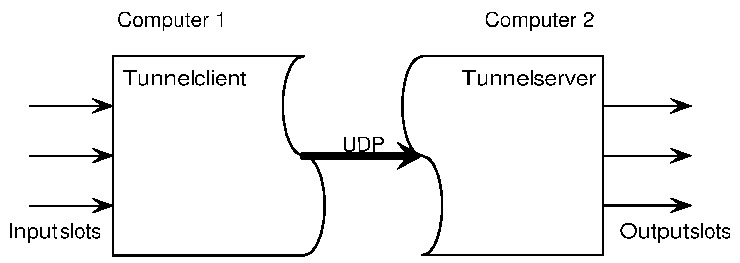
\includegraphics[width=8cm]{pics/tunnel}
%\caption{Tunnel component}
%\label{tunnel_pic}
\end{center}
%\end{figure}

An instance of the tunnel component either represents the input part
(client) or the output part (server). Value changes on the client are
then propagated via UDP datagrams to the server. When creating either
side of the tunnel you have to define the name and type of the slots
that should be created. The slot types of the client and the server
should always match.

\note{ArraySlots are currently not supported.}

\begin{classdesc}{Tunnel}{name = "Tunnel",\\ 
			  server = False, \\
                          slots = None, \\
                          port = 64738, \\
                          host = "localhost", \\
			  gather_messages = False, \\
                          verbose = False, \\
                          auto_insert = True}

\var{server} determines which end of the tunnel is created. The server is
always the ``end'' of a tunnel, i.e. where the values leave the
tunnel.  

\var{slots} specifies the slots to create on the tunnel. It
must be a list of 2-tuples containing two strings. The first string is
the name of the attribute and the second contains the type and
initializer of the slot (in Python syntax). The order and types of the
slots on the client and server should always match.  

\var{port} is the port number to use for the data transfer. The server
listens on this port and the client sends its data to this port on the
target machine.

\var{host} is a string containing the name or IP address of the target
machine where the server part of the tunnel is located. This parameter
is only used on the client side.

\var{gather_messages} determines whether value change messages should be
gathered and sent as one single message or not. If this flag is \code{False},
a message will be sent to the server whenever the value of a slot changes.
However, sometimes it may be the case that you can guarantee that all slots
will change their value at the same time. In such cases, you can set 
\var{gather_messages} to \code{True} which will have the effect that all
messages are collected and delayed until the {\em last} slot receives its 
new value. Only then will the value changes be sent as one big message
which increases the network performance.

If you set \var{verbose} to \code{True} the component will print some
messages so you can follow what it is doing.

\end{classdesc}


Here is an example of a sphere whose position is controlled by a remote
machine:

\begin{verbatim}
# Server code (machine A):

# Create a sphere...
s = Sphere()

# ...and the end of a tunnel that has one Vec3Slot called "pos"
t = Tunnel(
    server = True,
    slots = [("pos", "Vec3Slot()")]
)

# Connect the tunnel slot with the position of the sphere
t.pos_slot.connect(s.pos_slot)
\end{verbatim}

Execute this script with the viewer tool on machine A:

\begin{verbatim}
viewer.py server.py
\end{verbatim}

On the remote machine (the client) you can set the position of the above
sphere with the following code:

\begin{verbatim}
# Client code (machine B):

from cgkit import *

# Create the "entrance" of the tunnel...
t = Tunnel(
    slots = [("pos", "Vec3Slot()")],
    host = "<name or IP of machine A>"
)

# Move the sphere to position (1,0,0)
t.pos_slot.setValue(vec3(1,0,0))
\end{verbatim}

You can call this script by invoking it directly on machine B:

\begin{verbatim}
python client.py
\end{verbatim}

Calling the client code will move the sphere in the first program to 
the position (1,0,0). 

\begin{notice}[note]
As the underlying transport mechanism is using UDP datagrams there is no
error reporting mechanism. The client has no chance of knowing whether
a value change was properly propagated to the server or not. So if you
encounter any problems such as the sphere in the above example {\em not}
moving to another position, you can set the \var{verbose} flag to \code{True}
and additionally check the following points:

\begin{itemize}
\item Do the port numbers on the client and server match?
\item Did you specify the correct host name (or IP address) on the client side?
\item Is there a firewall blocking the network traffic?
\item Did you set \var{gather_messages} to \code{True} and the last slot 
  does not receive any new values? (try to set \var{gather_messages} to
  \code{False})
\end{itemize}

\end{notice}
